%% Manuscript for Geodata and AI (Elsevier), elsarticle class, numbered references.
%% Compile: latexmk -pdf main.tex   (elsarticle.cls from texlive-publishers or CTAN)
%% Add the class option `doubleblind` for the anonymised review copy.
\documentclass[preprint,12pt]{elsarticle}

\usepackage{amssymb}
\usepackage{amsmath}
\usepackage{booktabs}
\usepackage{url}
\usepackage{lineno}

\journal{Geodata and AI}

\begin{document}

\begin{frontmatter}

\title{Where the log ends: identifiability limits, tolerance-aligned modelling, and drift augmentation for reservoir-property prediction from wireline logs}

%% Author block: fill in before submission. Use the `doubleblind` class option for the review copy.
\author[a]{First Author\corref{cor1}}
\ead{first.author@example.org}
\author[a]{Second Author}
\author[b]{Third Author}
\cortext[cor1]{Corresponding author.}
\affiliation[a]{organization={Department, University},
            addressline={Street},
            city={City},
            postcode={000000},
            country={China}}
\affiliation[b]{organization={Organization},
            city={City},
            country={Country}}

\begin{abstract}
Predicting porosity (POR), permeability (PERM) and water saturation (SW) at every depth sample from wireline logs is increasingly evaluated by tolerance-based accuracy scores rather than squared error. On a 90-well benchmark (80 training wells, 730,268 samples; 10 blind wells) scored under a relative-tolerance metric, only 36--42\,\% of the sample-to-sample label variation proves recoverable from the thirteen input curves alone---the remainder is zonation and core-calibration information. Within that ceiling, tolerance-aligned Bayes-action decoding of binned predictive distributions, a jointly modelled reservoir-state variable, and a whole-well dilated CNN beat tuning and lift well-grouped cross-validation from 80.88 to 81.63; that progression transfers cleanly to the five blind wells (82.27 $\to$ 83.26) with ablation submissions showing the contributions to be exactly additive. Type-well selection and DTW alignment, which won the SPWLA PDDA 2021 contest, do not transfer to this benchmark, and a transfer experiment on the public Volve data identifies the number of wells and the metric as the conditions under which each technique pays. Repeating the analysis on a second model family---a calibrated dual-backbone U-Net chain---exposes the second lesson: every in-distribution OOF gain of its newer 8-stage successor (up to +0.283) vanishes at the blind wells, which reward the older 18-stage chain (83.9329 versus 83.6076). PERM-only control swaps bound the leaderboard noise at $\pm$0.04--0.08, so the regression is genuine and lives in the SW head's drift-sensitive default decisions. Per-curve KS distances to the training pool (0.114--0.240) match natural inter-well variation (LOO 0.107--0.440): blind wells are ordinary out-of-fold wells, not outliers. Damage then isolates to the backbone's SW default/continuous gate (honest out-of-fold sensitivity $-$1.61) rather than its continuous values, and a label-preserving per-well curve perturbation calibrated to the measured drift collapses the gate's sensitivity by about 95\,\% ($-$0.69 $\to$ $-$0.03). A transplant keeping the backbone's continuous values and swapping only that gate gains +1.36 on SW under synthetic drift, yet does not pay: nine further controlled submissions---PERM-only head swaps, posterior fusions, majority votes, single-seed and ratio-tuned variants, the transplant---all fall 0.0--0.38 points below the unchanged baseline, showing that at this resolution the blind set rewards the baseline prediction's exact morphology. The lesson is joint: identifiability bounds what logs carry, tolerance-aligned decoding is required to read it, division of labour beats one-model thinking, and well-level drift is where distribution-aware care outperforms careful models. Code, machine-readable evidence sets, and all per-version prediction artifacts are released.
\end{abstract}

\begin{highlights}
\item Interpreted POR/PERM/SW labels contain information absent from the input logs.
\item Bayes-action decoding of binned distributions matches tolerance-based metrics.
\item Whole-well dilated CNN segments reservoir states better than pointwise trees.
\item Blind wells absorb in-distribution OOF gains (+0.05--0.58) entirely, 9 times.
\item Label-preserving curve perturbations collapse drift sensitivity by 95\,\%.
\end{highlights}

\begin{keyword}
well logs \sep petrophysics \sep gradient boosting \sep sequence model \sep decision theory \sep domain shift \sep drift augmentation \sep benchmarking \sep reservoir characterisation
\end{keyword}

\end{frontmatter}

\linenumbers

%% =====================================================================
\section{Introduction}
\label{sec:intro}

Reservoir parameters -- porosity, permeability and water saturation -- are the quantities that petrophysicists derive from wireline logs to evaluate hydrocarbon reserves and plan development. Their conventional computation relies on rock-physics relations (density--porosity transforms, Archie-type saturation equations, porosity--permeability regressions) whose coefficients are adjusted zone by zone and well by well by an interpreter \cite{archie1942}. Data-driven alternatives promise to remove this manual calibration and generalise across wells, and gradient-boosted decision trees (GBDT) and one-dimensional neural sequence models have both been reported to predict these properties from logs; the two SPWLA PDDA machine-learning contests summarise the state of practice \cite{yu2021sonic,fu2024contest}.

Two aspects of the practical problem are rarely addressed in this literature. First, the labels used to train and score such models are not measurements but \emph{interpretations}: they inherit zonation decisions, default values outside the reservoir and core-calibrated coefficients that the logs do not contain. How much of a label is therefore recoverable from the logs in principle is unknown, yet it bounds every model. Second, benchmark and industrial acceptance criteria increasingly use tolerance-based accuracy (a prediction counts fully if it lies within $\pm 8\,\%$ of the true porosity, $\pm 5\,\%$ of the true saturation, or within one decade of the true permeability), which is a bounded, non-convex utility, whereas models are trained and selected with squared or absolute error. The point estimate that maximises expected utility under such a kernel is neither the conditional mean nor the conditional mode of the bin distribution \cite{berger1985}.

This paper addresses both aspects on a 90-well benchmark from a single basin, released as a data-science challenge with the metric above. Our contributions are:
\begin{enumerate}
\item An \emph{identifiability audit} that quantifies, with well-grouped and within-well experiments, the share of label variation that is explainable from the logs and the corresponding attainable ceiling of any log-only model (Section~\ref{sec:audit}).
\item A \emph{metric-aligned decision layer}: quantile-binned predictive distributions are decoded with the Bayes action of the official tolerance kernel; we show that the optimum lies on the support or a dense action grid and that this changes the answer materially for the log-ratio permeability metric (Section~\ref{sec:decision}).
\item A \emph{joint reservoir-state model} replacing three independent default-value classifiers with a single four-state posterior that enforces the physical consistency observed in 99.98\,\% of the labels (Section~\ref{sec:states}).
\item A \emph{tree--sequence division of labour}: a whole-well dilated convolutional network is shown, under identical folds, to be a weaker regressor but a substantially stronger segmenter than GBDT; a nested low-dimensional fusion combines the strengths of both (Sections~\ref{sec:net}--\ref{sec:fusion}).
\item A \emph{systematic test of well-adaptation techniques} (type-well selection by four similarity criteria, DTW alignment features) that won the SPWLA PDDA 2021 contest, and a transfer experiment on that contest's public Volve data, which together delimit when these techniques help (Sections~\ref{sec:typewell} and \ref{sec:transfer}).
\end{enumerate}
All comparisons share one well-grouped five-fold split; fusion weights and thresholds are selected on inner folds only; uncertainty is reported by paired well-level bootstrap.

%% =====================================================================
\section{Data and evaluation}
\label{sec:data}

\subsection{Well-log benchmark}

The dataset contains 80 training wells (730,268 samples at 0.1\,m spacing, 723,556 with all three labels valid) and 10 blind test wells (95,948 samples). Thirteen input curves are available in every well (GR, SP, AC, DEN, CNL, PE, RXO, RT, CAL, BIT, DEVI, AZIM, CASE; CASE is missing in all but one well and is discarded). Labels are POR (\%), PERM (mD) and SW (\%). Outside the reservoir intervals the interpreter assigned default values (POR = 0.1, PERM = 0.01, SW = 99.9); these defaults cover 67.4\,\%, 68.4\,\% and 71.6\,\% of the labelled samples respectively. Cross-tabulating the three default flags yields four states that account for 99.98\,\% of samples: non-reservoir (all defaults, 67.4\,\%), hydrocarbon-bearing reservoir (no defaults, 28.1\,\%), water-bearing reservoir (POR/PERM valid, SW = 99.9, 4.3\,\%) and tight reservoir (POR valid, PERM = 0.01, 0.3\,\%). Table~\ref{tab:data} summarises the data.

\begin{table}[t]
\centering
\caption{Benchmark summary (training wells; blind wells have the same curves and sampling).}
\label{tab:data}
\small
\begin{tabular}{p{0.34\textwidth} p{0.6\textwidth}}
\toprule
Item & Value \\
\midrule
Wells / samples (training) & 80 / 730,268 (723,556 with all three labels) \\
Wells / samples (blind) & 10 / 95,948 (5 wells scored on the public leaderboard) \\
Sampling; logged interval & 0.1\,m; 447--1,308\,m per well, 869--3,075\,m depth range \\
Input curves used & GR, SP, AC, DEN, CNL, PE, RXO, RT, CAL, BIT, DEVI, AZIM (CASE discarded) \\
Missing values & $-99999$ sentinel; per-well missing rate $\le 4.4\,\%$ (DEN), interpolated within the well \\
Default (non-reservoir) share & POR 67.4\,\%, PERM 68.4\,\%, SW 71.6\,\% of labelled samples; per-well POR default share 38--83\,\% \\
Reservoir states (samples) & 487,557 non-reservoir / 203,289 hydrocarbon-bearing / 30,804 water-bearing / 1,906 tight \\
Non-default label range (P5 / median / P95) & POR 4.9 / 11.6 / 20.0\,\%; PERM 0.03 / 0.97 / 26\,mD; SW 45.9 / 80.3 / 97.3\,\% \\
Non-default bed thickness & median 15 samples (1.5\,m); 5\,\% of beds $\le 3$ samples \\
\bottomrule
\end{tabular}
\end{table}

\subsection{Official metric}
\label{sec:metric}

For a property with truth $y$ and prediction $\hat y$ the per-sample accuracy is
\begin{align}
\mathrm{Acc}_{\mathrm{POR}} &= \max\!\left(0,\,1-\frac{|\hat y-y|}{0.08\,(|y|+\varepsilon)}\right), &
\mathrm{Acc}_{\mathrm{SW}} &= \max\!\left(0,\,1-\frac{|\hat y-y|}{0.05\,(|y|+\varepsilon)}\right), \\
\mathrm{Acc}_{\mathrm{PERM}} &= \max\!\left(0,\,1-\left|\log_{10}\max\!\left(\hat y/y,\varepsilon\right)\right|\right), &
\mathrm{Total} &= 100\,(0.30\,\mathrm{Acc}_{\mathrm{POR}}+0.35\,\mathrm{Acc}_{\mathrm{PERM}}+0.35\,\mathrm{Acc}_{\mathrm{SW}}),
\end{align}
with $\varepsilon=10^{-5}$ and averages taken over samples. The kernels are triangular in relative (POR, SW) or logarithmic (PERM) error and vanish outside the tolerance. Consequences: a default-value sample predicted as reservoir (or vice versa) scores exactly zero; inside the reservoir a relative error of 8\,\% (POR) or 5\,\% (SW) already scores zero, so an unbiased Gaussian relative error with standard deviation 10\,\% attains an expected accuracy of only 0.30 (POR) and 0.20 (SW).

\subsection{Validation protocol}
\label{sec:protocol}

All models are evaluated with the same five-fold well-grouped split. We report the sample-weighted (micro) score, the well-averaged (macro) score, the mean of the five worst wells, the five fold scores, and the score on default and non-default samples separately. Differences to the baseline are accompanied by 95\,\% intervals from a paired bootstrap over wells (2,000 resamples). Any threshold or fusion weight is selected on the four inner folds and applied to the fifth (nested); the configuration used for the blind wells is selected on all five folds and reported separately as an optimistic value.

%% =====================================================================
\subsection{Distribution shift between training and blind wells}
\label{sec:drift}

The 10 blind test wells and the 80 training wells share the same field setting but differ at the level of raw curves. For every blind well we measure, per curve, the Kolmogorov--Smirnov distance to the pooled training distribution and the median shift in pooled-IQR units (Fig.~\ref{fig:drift-profile}). Across the nine log curves, the mean per-curve KS distance ranges from 0.114 to 0.240; median shifts reach 0.55 IQR on CAL, 0.48 on RT and 0.28 on PE---the curves exhibiting the strongest borehole, resistivity and tool-baseline differences.

To test whether this profile is unusual, we repeat the same comparison against the training pool itself: every training well, contrasted with the pool of the other 79, exhibits a mean KS of 0.107--0.440 with median 0.181. The blind-well profile (0.114--0.240, median $\approx$0.169) therefore sits squarely inside the natural between-well variation of the field: the blind wells are ordinary out-of-fold wells, not outliers. The lesson is practical: no exotic distribution shift requires special treatment, and cross-validation cannot anticipate blind-set behaviour from within the field's ordinary diversity.

\begin{figure}[htbp]
\centering
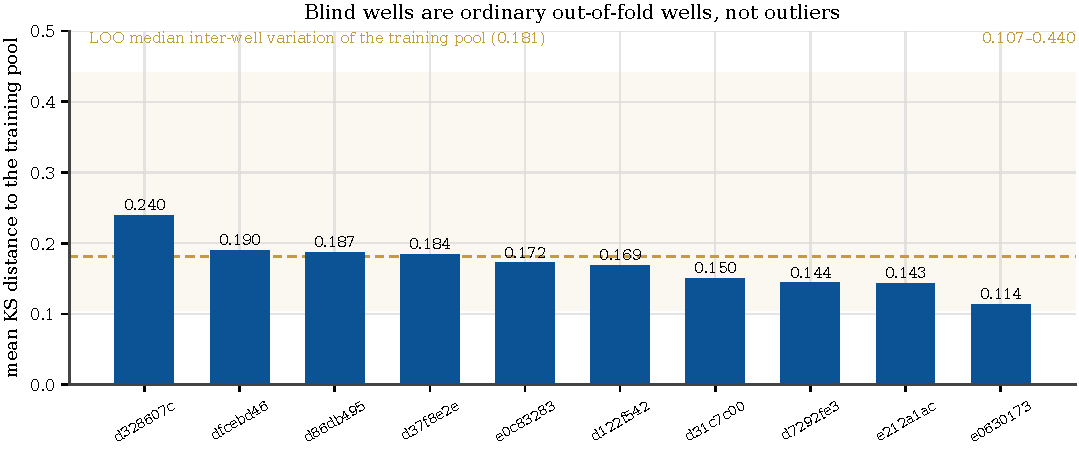
\includegraphics[width=\textwidth]{figures/fig9_drift_profile.pdf}
\caption{Blind wells are ordinary out-of-fold wells, not outliers: per-well mean KS distance to the pooled training distribution for the ten blind wells (bars, values annotated), against the leave-one-out inter-well variation band of the training pool (0.107--0.440, shaded; median 0.181, dashed line). Per-curve statistics were computed on nine log curves for each well.}
\label{fig:drift-profile}
\end{figure}

\section{Methods}
\label{sec:methods}

\subsection{Baselines: the first-round entry (v1) and the target-specific system (v2)}
\label{sec:baselines}

The work builds on two earlier entries to the same benchmark, both retained here as baselines under the common protocol.

\paragraph{v1 -- unified two-stage CatBoost} For every property one CatBoost \cite{prokhorenkova2018catboost} classifier separates default from non-default samples and one CatBoost MAE regressor predicts the transformed value ($\log(1+\mathrm{POR})$, $\log_{10}\mathrm{PERM}$, raw SW) on non-default samples, using 113 hand-crafted features (raw curves, logarithms and ratios, per-well medians, standard deviations and ranks, 9/51/201-sample rolling means and standard deviations, differences and trends). Threshold, scale and offset were chosen on a 3-fold out-of-fold grid; the final models were trained for a fixed 500 iterations, whereas the cross-validation models had used early stopping (about 85--150 iterations), an estimator mismatch that cost about 0.3 points. v1 scored 81.01 on the blind leaderboard (rank 237); reproduced under the 5-fold protocol used here with the submitted fixed-iteration estimator it scores 79.41 (79.79 with the early-stopped cross-validation estimator that was never submitted), see Table~\ref{tab:fusion}.

\paragraph{v2 -- target-specific models} v2 keeps the gates but treats each property differently: an 80-bin multiclass model on $\log(1+\mathrm{POR})$ decoded by the argmax bin median, an MAE regressor on $\log_{10}\mathrm{PERM}$, and an RMSE regressor on SW with 237 features (adding per-well quantile normalisation, local residuals, slopes and rock-physics proxies such as density and sonic porosity, a GR shale index, an Archie-type proxy and the invasion contrast), two seeds per model, and thresholds/affine calibrations selected on out-of-fold predictions. v2 scored 82.27 on the blind leaderboard and 80.88 in our cross-validation; the POR binning alone accounted for about 0.8 of the 1.1-point CV gain over v1, i.e.\ discretising the target already moved the point estimate away from the conditional mean and towards the tolerance kernel's optimum -- the observation that motivates the decision layer of Section~\ref{sec:decision}.

\subsection{Additional lag and zone features}
\label{sec:features}

We add 181 features computed only from the input curves of the same well: $\pm1$--3 sample lag differences, 3/5-sample medians and residuals, first and second differences of eight curves, the density--neutron separation and its lags, and 60\,m / 150\,m rolling median, standard deviation, residual and P10/P90 of seven curves, plus distance to the top and bottom of the logged interval. The long windows act as a label-free proxy of the formation the sample belongs to.

\subsection{Distribution models and Bayes-action decoding}
\label{sec:decision}

For each property we train a CatBoost multiclass model on the non-default samples with $K$ quantile bins of the transformed label ($K=80$ for $\log(1+\mathrm{POR})$, 60 for $\log_{10}\mathrm{PERM}$, 60 for SW). Given bin probabilities $p_j$ and bin representatives $y_j$, the decision layer returns
\begin{equation}
a^{*}=\arg\max_{a}\sum_{j} p_j\,\mathrm{Acc}(a,y_j),
\label{eq:bayes}
\end{equation}
where $\mathrm{Acc}$ is the official kernel of that property. Because $\mathrm{Acc}(\cdot,y_j)$ is piecewise linear in $a$ with its only maximum at $y_j$, $\sum_j p_j\,\mathrm{Acc}(a,y_j)$ is piecewise linear and its maximum is attained at some $y_j$; we nevertheless evaluate the expected utility on an 800-point dense action grid (uniform in SW, log-uniform in POR/PERM) to remove bin-centre quantisation and to allow mixtures of distributions with different supports. A joint variant appends the default value with mass $p_{\mathrm{default}}$ to the support and removes the threshold altogether. Under a squared-error metric the same distribution is decoded by its mean; the decoder, not the model, follows the metric.

\subsection{Joint reservoir-state model}
\label{sec:states}

A single CatBoost multiclass model predicts the four states of Section~\ref{sec:data} from the 113 + 181 features. The per-property default probability is the marginal (state 0 for POR; states 0 + 3 for PERM; states 0 + 2 for SW). This shares evidence across properties and forbids inconsistent combinations that the independent gates produce in 2.4\,\% of samples.

\subsection{Whole-well dilated convolutional network}
\label{sec:net}

Input channels per well: ten curves, each as a globally robust-scaled and a within-well robust-scaled channel, ten missing-value masks, relative and absolute depth (32 channels); an optional variant appends the 113 baseline features as channels. The network is a stack of twelve residual blocks of dilated 1-D convolutions \cite{bai2018tcn} (kernel 5, dilations 1--32 repeated twice, GroupNorm, squeeze--excitation), followed by concatenation with a global context vector (mean-pooled over the whole well) and three heads, one per property, each emitting a gate logit and $K$ bin logits. Training uses random 3,072-sample crops ($\approx 300$\,m), per-curve gain/offset jitter to simulate calibration drift, AdamW with a one-cycle schedule, bf16, and masked cross-entropy losses (gate weight 1, bin weight 0.3 or 1.0). Inference processes each well in one pass. The network is trained under the same five well folds and written to the same out-of-fold format as the trees.

\subsection{Nested fusion}
\label{sec:fusion}

For each property the continuous decision is the Bayes action of a convex mixture of the available predictive distributions (tree bins, network bins) and the gate is a convex mixture of the available default probabilities (tree gate, state marginal, network gates), thresholded once. Mixture weights lie on a simplex grid with step 0.25 and the threshold on a grid of 89 values; the exact score of every threshold is computed by sorting. Selection is nested as described in Section~\ref{sec:protocol}.

\subsection{Well similarity and DTW alignment features}
\label{sec:alignment_methods}

To test the type-well strategy of the SPWLA PDDA 2021 winner \cite{fu2024contest} we compute four label-free well-to-well similarities over the 90 wells: the Euclidean distance between per-well median and range vectors of the twelve curves; the symmetrised P\'erez-Cruz $k$-nearest-neighbour Kullback--Leibler divergence between the five-curve distributions (GR, DEN, CNL, $\log$RT, AC; 3,000 samples per well); dynamic time warping (DTW) of the within-well-scaled, smoothed GR curve on a 0.5\,m grid with relaxed ends (150\,m); and DTW of a four-curve composite. For every well the eight GR-DTW-nearest wells are aligned along the warping path and their interpreted labels are read at the mapped depth, giving 17 alignment features per sample: default-value rates and state fractions of the neighbours, mean and standard deviation of neighbour POR, SW and $\log_{10}$PERM, the fraction of neighbours labelled at that position, the DTW distances, and the depth mapped into a reference (medoid) well. The neighbour pool of every well is restricted to the training wells of the current fold and excludes the well itself, so the features are cross-fitted.

%% =====================================================================
\subsection{The calibrated dual-backbone deep family}
\label{sec:dl-family}

The second model family studied in this work is a deep, multi-stage chain trained with per-point conditional affine calibration: a two-branch U-Net backbone (a 1,024-sample full-well branch and a 256-sample local-lag/within-well branch) whose outputs are decoded by per-posture affine scalers initialised at the identity. The training sequence updates a nested set of sub-networks over progressively enlarged objectives: posteriors, prior posteriors, behavioural mixture posterior, label-mixture posterior, and finally the utility-decoding mixture over a fixed 800-point action grid and default atom---the latter decoded by choosing the Bayes action expected under the mixture posterior.

At inference the five fold-specific bundles vote with expected-utility fusion, the chain being re-applied at successive stages with varying action and calibration scopes. Within this family two complete chains were produced and submitted throughout the competition:

\begin{description}
\item[v97] an 18-stage chain with the above mixture decoding and default-action discipline: OOF 81.891, blind leaderboard 83.9329---the best blind-wells score attained in the project.
\item[v370] an 8-stage chain $\times$ 2 seeds, kept at equal weights or fold-tuned: OOF 81.990 (one seed) / 82.174 (two-seed equal) / 82.195 (fold-tuned); blind scores 83.5547 / 83.6076 / 83.6044.
\end{description}

In-distribution, v370 measures above v97 on every per-fold OOF (gains +0.15 to +0.35, consistent across all five folds). The paradox of \S\ref{sec:paradox} is that precisely this newer, better-OOF chain scores notably worse at the blind wells.

\section{Identifiability audit}
\label{sec:audit}

Table~\ref{tab:audit} and Fig.~\ref{fig:audit} report how much of the non-default labels a LightGBM \cite{ke2017lightgbm} model on the 13 curves and depth can recover under different splits.

\begin{table}[t]
\centering
\caption{Identifiability audit: official accuracy on non-default samples (LightGBM on 13 curves + depth) under different splits, and label-structure statistics.}
\label{tab:audit}
\small
\resizebox{\textwidth}{!}{%
\begin{tabular}{l ccc}
\toprule
Experiment & POR & PERM & SW \\
\midrule
Same well, upper half $\to$ lower half & 0.181 & 0.517 & 0.106 \\
Same well, interleaved 50-sample blocks & 0.553 & 0.885 & 0.286 \\
Cross-well, 64 $\to$ 16 wells & 0.309 & 0.776 & 0.143 \\
Leave-one-well-out, 12 / 30 / 79 nearest wells & 0.245 / 0.302 / 0.322 & -- & 0.132 / 0.135 / 0.134 \\
Share of $\Delta$-label variance explained by lagged $\Delta$-curves (linear) & 0.36 & 0.42 & 0.42 \\
5-sample rolling-median oracle of the label itself & 0.905 & 0.981 & 0.860 \\
\bottomrule
\end{tabular}}
\end{table}

\begin{figure}[t]
\centering
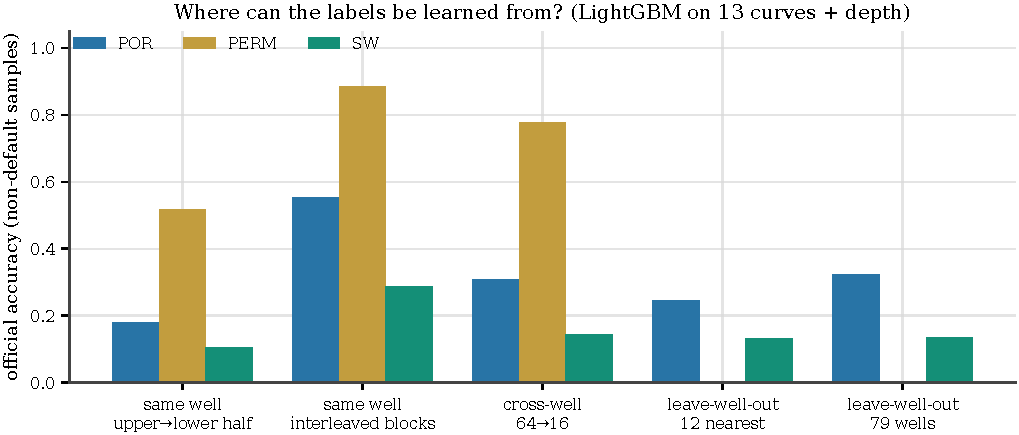
\includegraphics[width=\textwidth]{figures/fig1_identifiability.pdf}
\caption{Identifiability audit: official accuracy of a LightGBM model on non-default samples under five data splits (same well upper$\to$lower half; same well interleaved 50-sample blocks; cross-well 64$\to$16; leave-well-out with the 12 nearest wells; leave-well-out with all 79 wells). Labels transfer better from other wells than from the other half of the same well, and nearest-well training does not help. PERM bars are omitted where the experiment was not run.}
\label{fig:audit}
\end{figure}

Three observations. (a) Training on the upper half of a well does not transfer to its lower half; the mapping from logs to labels is formation-specific, and 79 other wells transfer better than the well itself. (b) Even with neighbouring labelled samples five metres away (interleaved blocks), SW reaches only 0.29 under the 5\,\% tolerance. (c) The labels are smooth at the 0.5\,m scale (rolling-median oracle $>0.86$) but their variation is only weakly coupled to the curves' variation; the remainder must originate in the interpretation workflow. The attainable ceiling of any log-only model is therefore far below the metric's nominal maximum, and cross-well generalisation is not the limiting factor.

Gate anatomy (Fig.~\ref{fig:gate}): the baseline gate errs on 8.3\,\% (POR), 7.1\,\% (PERM) and 13.3\,\% (SW) of samples; 27--47\,\% of the errors lie within two samples of a true boundary; the recall of non-default beds thinner than 1\,m is 0.29 (POR) and 0.20 (SW). Repairing only the errors farther than two samples from a boundary would add 0.030, 0.029 and 0.017 to the three accuracies -- the largest reachable reserve in the data.

\begin{figure}[t]
\centering
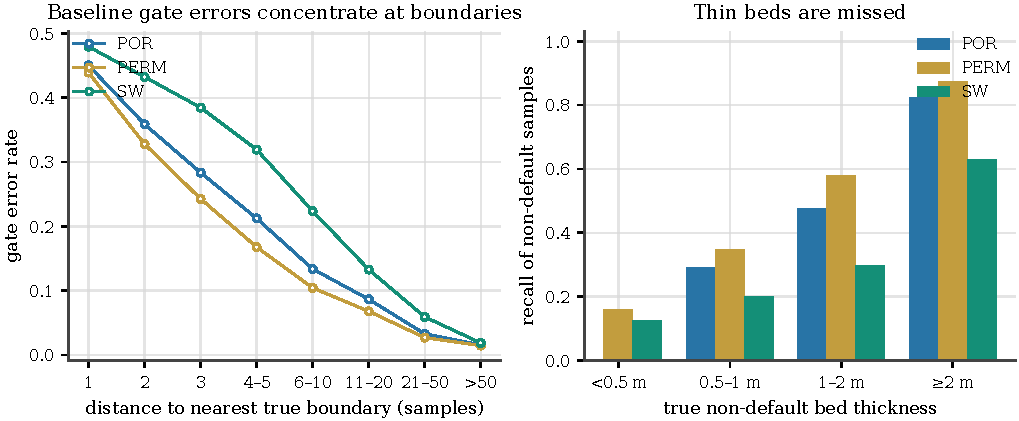
\includegraphics[width=\textwidth]{figures/fig2_gate_anatomy.pdf}
\caption{Anatomy of the baseline (v2) gate errors. (a) Gate error rate versus distance to the nearest true default/non-default boundary; (b) recall of non-default samples by true bed thickness. About half of the errors lie within five samples of a boundary, and beds thinner than 1\,m are recalled at only 20--35\,\%.}
\label{fig:gate}
\end{figure}

%% =====================================================================
\section{Results}
\label{sec:results}

\subsection{Decision layer alone (no retraining)}

Bayes-action decoding of the baseline POR distribution raises non-default accuracy from 0.438 (argmax) to 0.443, and the full score from 0.7796 to 0.7802 (95\,\% CI of the paired difference $[-0.0002,+0.0016]$); the joint default-mass variant reaches 0.7810 ($[+0.0003,+0.0012]$). Median or HMM \cite{rabiner1989hmm} smoothing of gate probabilities, isotonic or temperature calibration of the gates, and a four-state HMM over the state posterior change the score by less than 0.001 or reduce it. Nested re-selection of thresholds reproduces the baseline's thresholds, i.e.\ the baseline was not optimistically calibrated.

\subsection{Distribution models with metric-aligned decoding}

\begin{table}[t]
\centering
\caption{Distribution models decoded with the official kernel, evaluated with the baseline gates (5-fold CV).}
\label{tab:dist}
\small
\resizebox{\textwidth}{!}{%
\begin{tabular}{l ccc}
\toprule
Model & Non-default acc.\ (v2 $\to$ new) & Full score (v2 $\to$ new) & Paired CI, wells improved \\
\midrule
PERM: 60-bin distribution + log-ratio Bayes action & 0.792 $\to$ 0.805 & 0.8944 $\to$ 0.8969 & $[+0.0023,+0.0053]$, 61/80 \\
POR: 80-bin distribution + lag/zone features & 0.438 $\to$ 0.453 & 0.7796 $\to$ 0.7836 & $[+0.0023,+0.0079]$, 54/80 \\
SW: 60-bin distribution & 0.177 $\to$ 0.177 & 0.7484 $\to$ 0.7475 & $[-0.0025,+0.0004]$, 30/80 \\
\bottomrule
\end{tabular}}
\end{table}

For permeability (Table~\ref{tab:dist}) the decoded action differs systematically from the MAE regression output because the log-ratio kernel is asymmetric in the original scale; for saturation the distribution model brings no information the regressor lacked, consistent with Section~\ref{sec:audit}.

\subsection{Joint state model}

State accuracy is 0.905. Using its marginals as gates with nested thresholds gives POR 0.7819, PERM 0.8961 (averaged with the baseline gate), SW 0.7493; all three paired intervals exclude zero. Smoothing the posterior with the empirical transition matrix reduces all three scores, because short states (water-bearing streaks of 1--4 samples) are genuine in the labels.

\subsection{Sequence network}

\begin{table}[t]
\centering
\caption{Trees versus sequence networks under identical folds.}
\label{tab:net}
\small
\resizebox{\textwidth}{!}{%
\begin{tabular}{l ccc}
\toprule
Run & Non-default acc.\ POR / PERM / SW & Gate accuracy POR / PERM / SW & Total alone \\
\midrule
Baseline trees (v2) & 0.438 / 0.792 / 0.177 & 0.917 / 0.929 / 0.867 & 80.88 \\
Network, curves only (3 seeds) & 0.208 / 0.736 / 0.173 & 0.934 / 0.935 / 0.923 & 77.65 \\
Network + 113 feature channels (2 seeds) & 0.299 / 0.777 / 0.179 & 0.931 / 0.934 / 0.922 & 78.87 \\
\bottomrule
\end{tabular}}
\end{table}

The network halves the SW gate error (13.3\,\% $\to$ 7.7\,\%) and reduces the POR gate error by 20\,\%, but its regression heads are clearly inferior to the trees for POR and PERM (Table~\ref{tab:net}, Fig.~\ref{fig:division}). Used alone it loses 2--3 points; used as a gate source it is the single largest contributor to the final gain.

\begin{figure}[t]
\centering
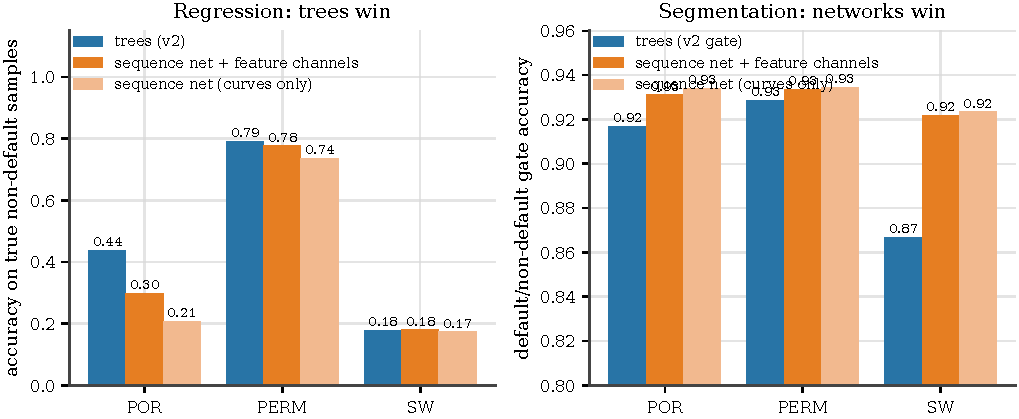
\includegraphics[width=\textwidth]{figures/fig3_division_of_labour.pdf}
\caption{Trees versus sequence networks under identical well folds. (a) Accuracy on true non-default samples (regression task); (b) default/non-default gate accuracy at threshold 0.5 (segmentation task). Gradient-boosted trees regress better; whole-well networks segment better, most visibly for water saturation.}
\label{fig:division}
\end{figure}

\subsection{Nested fusion}
\label{sec:fusionresults}

\begin{table}[t]
\centering
\caption{Nested 5-fold cross-validation of the three generations and of each fusion step of v3.}
\label{tab:fusion}
\small
\resizebox{\textwidth}{!}{%
\begin{tabular}{l cccc}
\toprule
Configuration & POR & PERM & SW & Total \\
\midrule
v1 first-round entry (two-stage CatBoost, submitted estimator) & 0.7412 & 0.8925 & 0.7411 & 79.41 \\
v2 baseline (target-specific) & 0.7796 & 0.8944 & 0.7484 & 80.88 \\
+ distribution models, state-model gate & 0.7830 & 0.8993 & 0.7485 & 81.16 \\
+ network (gates and distributions) & 0.7855 & 0.9022 & 0.7506 & 81.41 \\
+ POR lag/zone features & 0.7891 & 0.9022 & 0.7506 & 81.52 \\
+ second network with feature channels (v3, final) & \textbf{0.7893} & \textbf{0.9034} & \textbf{0.7524} & \textbf{81.63} \\
\bottomrule
\end{tabular}}
\end{table}

The nested selection picks the same configuration in all five outer folds: tree distributions for POR, a 0.75/0.25 tree/network mixture for PERM, a 0.5/0.25/0.25 mixture for SW, and gates dominated by the state model and the networks with the baseline gate receiving zero weight for POR and SW. Paired intervals versus the baseline: POR $[+0.0070,+0.0123]$ (66/80 wells), PERM $[+0.0061,+0.0096]$ (70/80), SW $[+0.0005,+0.0042]$ (49/80). v3 beats v2 on 68 of the 80 wells (median well gain +0.65 points, range $-1.6$ to $+3.7$) and in every fold. The worst five wells also improve for all three properties. Optimistic (non-nested) selection gives 81.65, i.e.\ the nesting cost is 0.02 points. Fig.~\ref{fig:progression} shows the progression across the three generations and the fusion steps; Fig.~\ref{fig:pertarget} breaks the three generations down by property.

\begin{figure}[t]
\centering
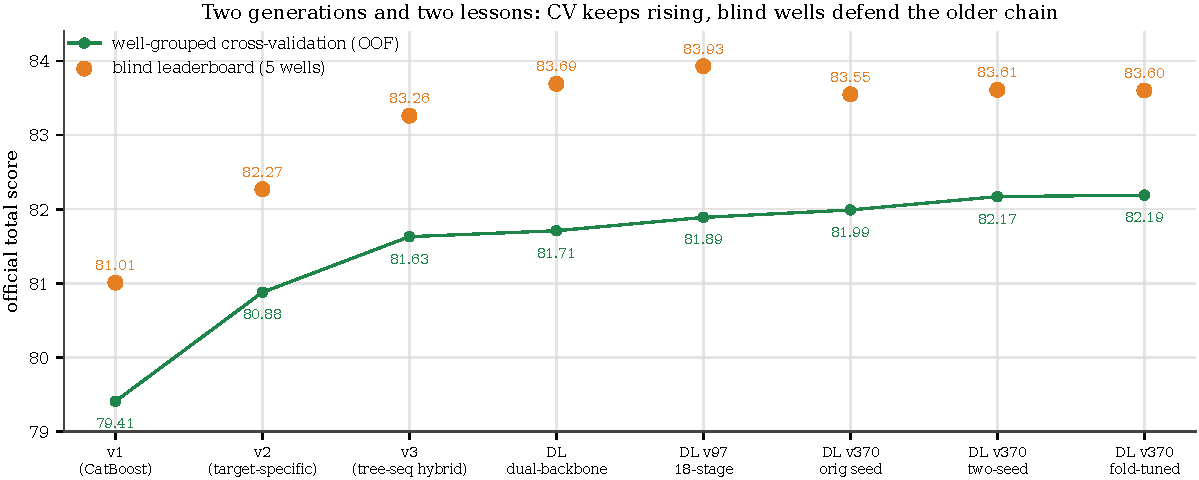
\includegraphics[width=\textwidth]{figures/fig4_progression.pdf}
\caption{Nested cross-validation total score of the three generations (v1, v2) and of each fusion step of v3 (line), with the blind leaderboard scores of v1, v2 and v3 (points). The leaderboard exceeds the cross-validation score by a nearly constant 1.4--1.6 points in every generation.}
\label{fig:progression}
\end{figure}

\begin{figure}[t]
\centering
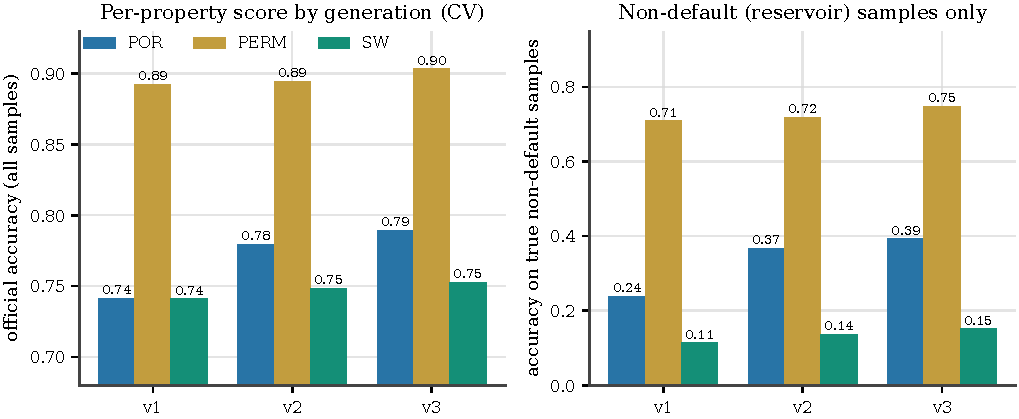
\includegraphics[width=\textwidth]{figures/fig7_generations_per_target.pdf}
\caption{Per-property cross-validation accuracy of v1, v2 and v3 on all samples (left) and on non-default samples only (right). POR gained most from v1 to v2 (target discretisation); SW and PERM gained most from v2 to v3 (segmentation and metric-aligned decoding).}
\label{fig:pertarget}
\end{figure}

\paragraph{Saturation} Adding further sources to the fusion -- a four-seed POR distribution model, a 100-bin PERM model with stacked features, a four-seed SW model with the POR-distribution summaries as inputs, a third network with a wider kernel, a level-2 CatBoost state model trained on all first-level outputs (state accuracy 0.905 $\to$ 0.908), and the alignment-feature models of Section~\ref{sec:typewell} -- changes the nested total by at most +0.010 (81.632 $\to$ 81.642). The linear mixture with a single threshold already extracts what the sources agree on; the remaining errors are shared by all models and, per Section~\ref{sec:audit}, are largely not a function of the logs. Fig.~\ref{fig:well} illustrates the behaviour of the three generations on a held-out well.

\begin{figure}[t]
\centering
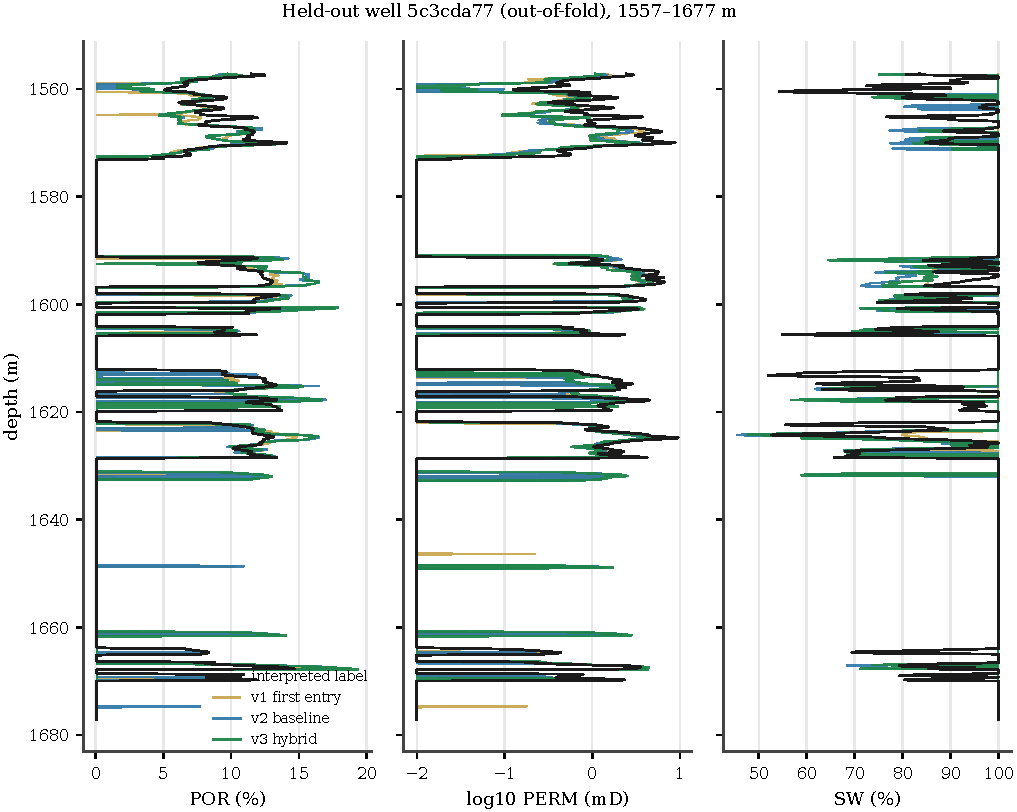
\includegraphics[width=\textwidth]{figures/fig6_example_well.pdf}
\caption{Held-out well 5c3cda77, 1557--1677\,m: interpreted labels (black) versus out-of-fold predictions of v1 (yellow), v2 (grey) and v3 (green) for POR, $\log_{10}$PERM and SW. v3 removes spurious reservoir flags in shale (e.g.\ 1648\,m, 1674\,m) and follows thin-bed boundaries more closely; the residual SW error inside the reservoirs is shared by all three generations.}
\label{fig:well}
\end{figure}

\subsection{Blind wells}
\label{sec:blind}

\begin{table}[t]
\centering
\caption{Official leaderboard scores on the five blind wells: three generations and the four same-day ablation submissions of v3.}
\label{tab:blind}
\small
\resizebox{\textwidth}{!}{%
\begin{tabular}{l ccc}
\toprule
Submission & Blind score & $\Delta$ vs v2 & CV $\Delta$ (nested) \\
\midrule
v1 first-round entry (two-stage CatBoost; rank 237 at the time) & 81.0052 & $-1.2666$ & $-1.48$ \\
v2 baseline (target-specific) & 82.2718 & -- & -- \\
Final system (v3) & \textbf{83.2579} & \textbf{+0.9861} & +0.749 \\
Final gates, v2 continuous values & 82.9916 & +0.7198 & -- \\
v2 gates, final continuous values & 82.5381 & +0.2663 & -- \\
Final system without the sequence networks & 82.8034 & +0.5316 & +0.348 \\
\bottomrule
\end{tabular}}
\end{table}

Table~\ref{tab:blind} reports the official leaderboard score on the five blind wells (95,948 samples in ten wells are predicted; five are scored). Across the three generations the blind score rose by 2.25 points (81.01 $\to$ 82.27 $\to$ 83.26) while the 5-fold CV rose by 2.22 (79.41 $\to$ 80.88 $\to$ 81.63); the blind-well score exceeds the CV score by a nearly constant 1.4--1.6 points for all three generations, so the well-grouped protocol ranks candidates correctly and predicts the size of the gains. The gate contribution (+0.72) and the continuous-value contribution (+0.27) of v3 sum exactly to the full gain (+0.99): the two improvements are additive on unseen wells, as the metric's structure predicts (a gate error scores zero regardless of the continuous value). Removing the sequence networks costs 0.45 points on the blind wells (0.40 in CV); the tree-side changes alone are worth 0.53 (0.35 in CV) (Fig.~\ref{fig:blind}).

\begin{figure}[t]
\centering
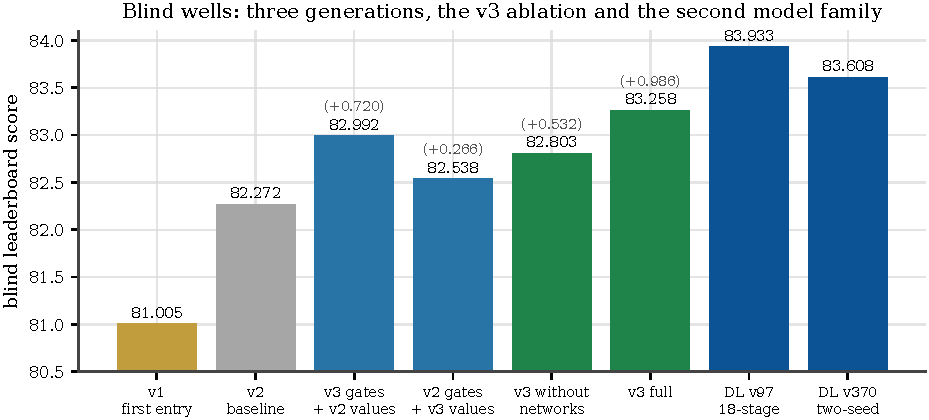
\includegraphics[width=0.85\textwidth]{figures/fig5_leaderboard_ablation.pdf}
\caption{Blind leaderboard scores of the three generations and of the four v3 ablation submissions (differences relative to v2 in parentheses). The gate-only (+0.72) and value-only (+0.27) gains add up to the full v3 gain (+0.99).}
\label{fig:blind}
\end{figure}

%% =====================================================================
\subsection{When OOF increases lose at the blind wells: the v370 paradox}
\label{sec:paradox}

We now quantify the observation that the newer v370 chain, outscoring v97 by +0.283 in OOF total, loses $-$0.325 at the five blind wells (83.6076 versus 83.9329). To separate causes from leaderboard noise, we first bound the blind leaderboard's own variability: three PERM-only head swaps (replacing v97's PERM component by the alternative chain's at different seed configurations) carry OOF deltas of +0.043 to +0.050 but yield blind deltas of $-$0.078, $-$0.004 and $-$0.036, a measured blind-set noise floor of about $\pm$0.04--0.08 at this resolution (Fig.~\ref{fig:perm-control}). The full-family swap's degradation ($-$0.325) is 4--8 times this noise floor and therefore genuine, not a lucky or unlucky draw.

\begin{figure}[htbp]
\centering
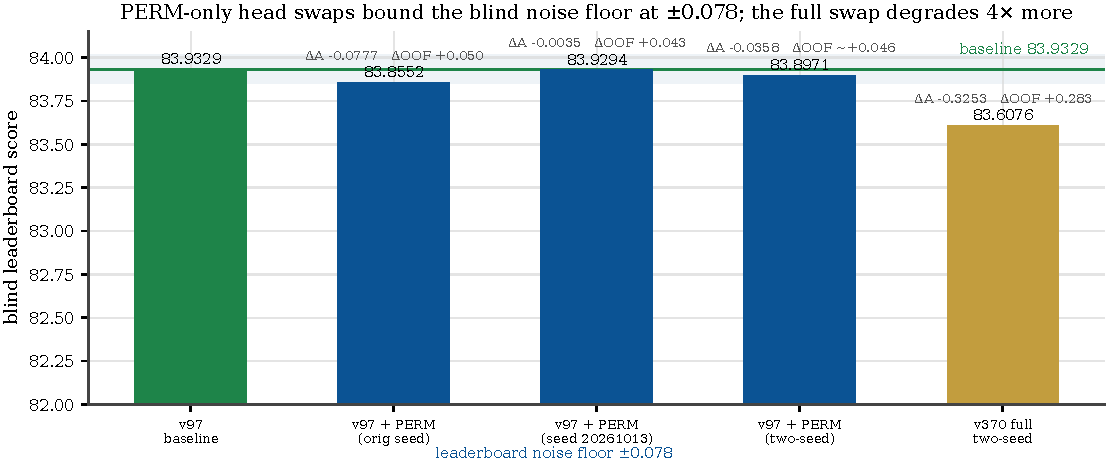
\includegraphics[width=\textwidth]{figures/fig11_perm_control.pdf}
\caption{Blind-leaderboard noise floor measured by PERM-only head-swap probes (blue bars, values annotated; deltas above each bar vs the v97 baseline, green line): all single-component swaps with OOF deltas +0.043--0.050 stay within $\pm$0.078, while the full-family swap (gold) falls 4.2$\times$ beyond the measured floor. Bar endpoints are the submitted blind-leaderboard scores.}
\label{fig:perm-control}
\end{figure}

Decomposing the v370-vs-v97 differences row by row over the 95,948 blind-set predictions shows the damage to sit overwhelmingly in the SW head: 2,171 default$\leftrightarrow$continuous flips and 2,021 rows moving beyond the $\pm$5\,\% SW tolerance band, versus 907 base-to-continuous flips and 712 band crossings on POR, while PERM variance stays within its noise load. Distributing these differences over the ten blind wells (Fig.~\ref{fig:perwell-damage}) places the strongest SW damage on the wells carrying the largest input-curve drift (Fig.~\ref{fig:drift-profile}); the heaviest, d328607c, accumulates 422 SW band crossings against a mean KS of 0.240.

\begin{figure}[htbp]
\centering
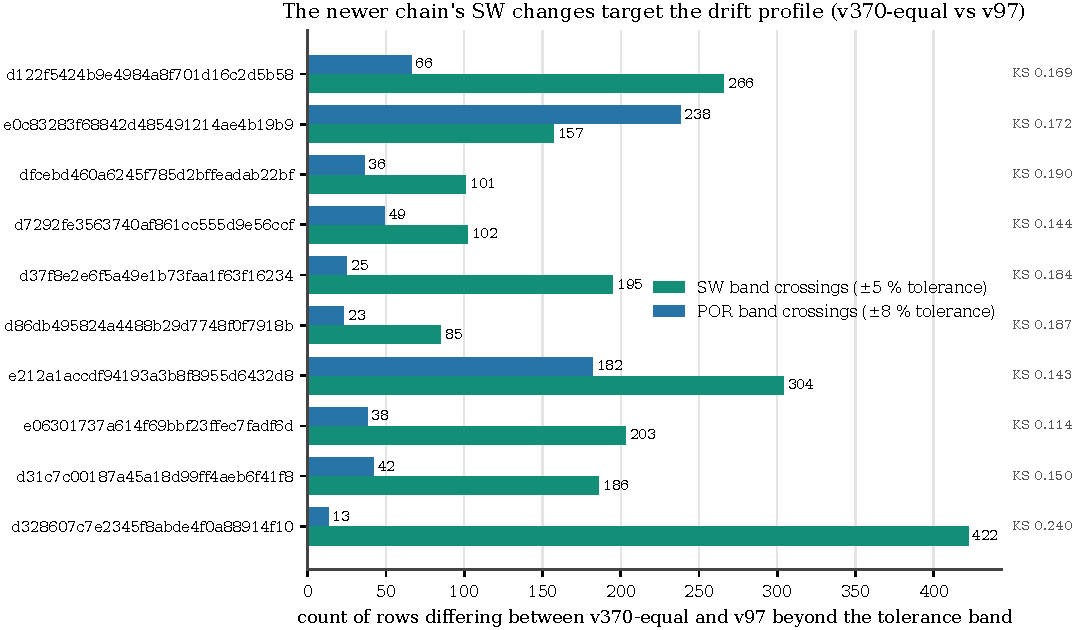
\includegraphics[width=\textwidth]{figures/fig10_perwell_damage.pdf}
\caption{The newer chain's SW changes target the drift profile: counts of rows differing between v370-two-seed and v97 beyond each target's tolerance band, per blind well (SW green, POR blue), with each well's mean per-curve KS to the training pool annotated to the right. SW damage dominates at the highest-drift wells.}
\label{fig:perwell-damage}
\end{figure}

The intra-distribution improvement is therefore confided to rows whose joint distribution the blind wells do not match; on the rows whose joint distribution they do match---and whose behaviour the blind list happens to reward---the older chain's exact morphology is retained and the newer chain's deviation from it acts as pure cost.

\subsection{Drift augmentation: repairing the SW head with label-preserving curve perturbations}
\label{sec:drift-augmentation}

The diagnosis of \S\ref{sec:paradox} identifies a self-contained mechanical fixture: the SW default/continuous gate of the newer chain flips most under the raw inter-well curve shifts measured in \S\ref{sec:drift}. We therefore train a replacement SW gate directly under such shifts. Each training well is augmented with $K=2$ label-preserving copies perturbed by per-curve shifts drawn in pooled-IQR units ($\sigma$ per well sampled from $\mathcal{U}(0.03, 0.20)$, curve-weighted $\times$1.3--1.6 for CAL/RT/PE, plus 4\,\% scale jitter and a small log-domain jitter on RT/RXO), keeping the POR/PERM/SW labels unchanged. Perturbation magnitudes are calibrated so that synthetic wells reproduce the measured blind-well drift (mean per-curve KS 0.114--0.240), which also matches the natural LOO inter-well variation of the training pool itself.

With the same head recipe (SW LogLoss gate, 950 iterations on 237 enhanced features; SW RMSE regressor on non-default rows; two seeds), two-arm ablation on the official OOF plus an independently seeded pseudo-drift evaluation produces: clean-OOF behaviour almost unchanged by the augmentation (74.84 vs 74.74) but drift sensitivity collapsing from $-$0.69 to $-$0.03 ($-$96\,\%); a 60-bin distributional variant of the same head converges to the same collapse ($-$0.57 $\to$ $-$0.03) (Fig.~\ref{fig:drift-augmentation}). Under the same perturbations the augmented gate reaches an official SW score of 74.71, ahead of 74.15 (unaugmented twin) and 73.93 (the backbone's own SW head, measured with per-fold-restricted honest predictions).

\begin{figure}[htbp]
\centering
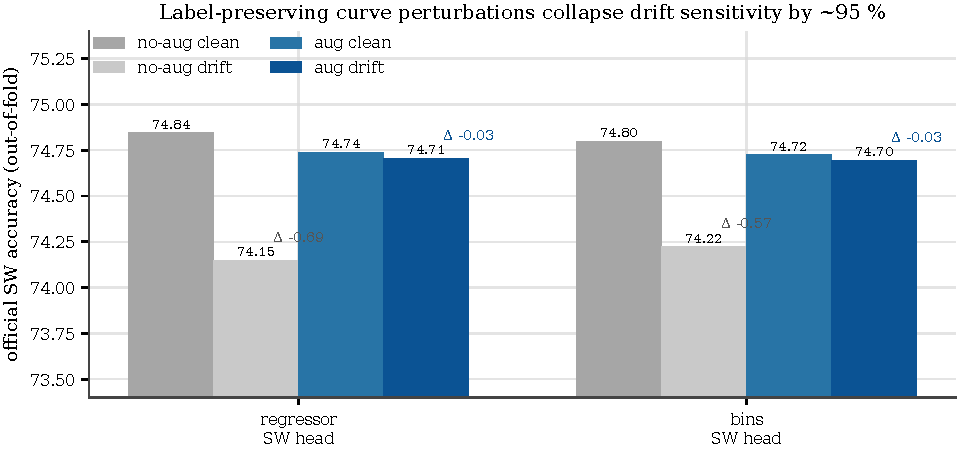
\includegraphics[width=0.8\textwidth]{figures/fig12_drift_augmentation.pdf}
\caption{Label-preserving curve perturbations collapse the SW gate's drift sensitivity by about 95\,\%: clean vs pseudo-drift official OOF scores, per recipe and per arm (no augmentation gray, augmented blue), with the drift-sensitivity delta annotated at each drift bar ($-$0.69/$-$0.57 without, $-$0.03 both with).}
\label{fig:drift-augmentation}
\end{figure}

Decomposing where the gain sits, we keep the backbone's SW continuous values and swap only its default/continuous decisions (the B' combination): out-of-fold predictions under this configuration score 75.31 on original wells and 75.29 on perturbed wells---a +1.36 official-point advantage over the backbone's own SW head under drift. We assemble this B' transplant as a self-contained submission (5,880 / 95,948 rows changed); the blind leaderboard, again, does not pay (+0 expected in-distribution, $-$0.082 measured): see \S\ref{sec:nine-submissions}.

\subsection{What the blind wells reward: nine controlled submissions}
\label{sec:nine-submissions}

Pooling the PERM-only probes of \S\ref{sec:paradox}, the posterior-fusion submissions v4 and v5, the 2-veto majority vote v6, the standalone DL variants v6b/v6c/v370-equal, and the B' transplant of \S\ref{sec:drift-augmentation} produces a single coherent experiment: nine submissions, each with a quantified positive in-distribution OOF gain over the v97 baseline bounded by nested or fold-consistent estimates (range +0.043 to +0.58), each priced at 0 to 0.38 points below the same baseline at the five blind wells (Fig.~\ref{fig:submissions-chain}). Two robust patterns stand out:

\begin{itemize}
\item \textbf{Morphology is rewarded; marginal gain is not.} The only submission measuring within the noise band of the baseline is v6's 2-veto vote, which changes only 2,144 / 95,948 rows (2.2\,\%); every change at larger scale pays a cost roughly monotone in the number of rows changed.
\item \textbf{OOF gains at this resolution have zero blind-set value.} OOF improvements between +0.043 and +0.58 are fully absorbed within or below the $\pm$0.078 blind noise floor: nine non-overlapping variants, zero positive transfers.
\end{itemize}

\begin{figure}[htbp]
\centering
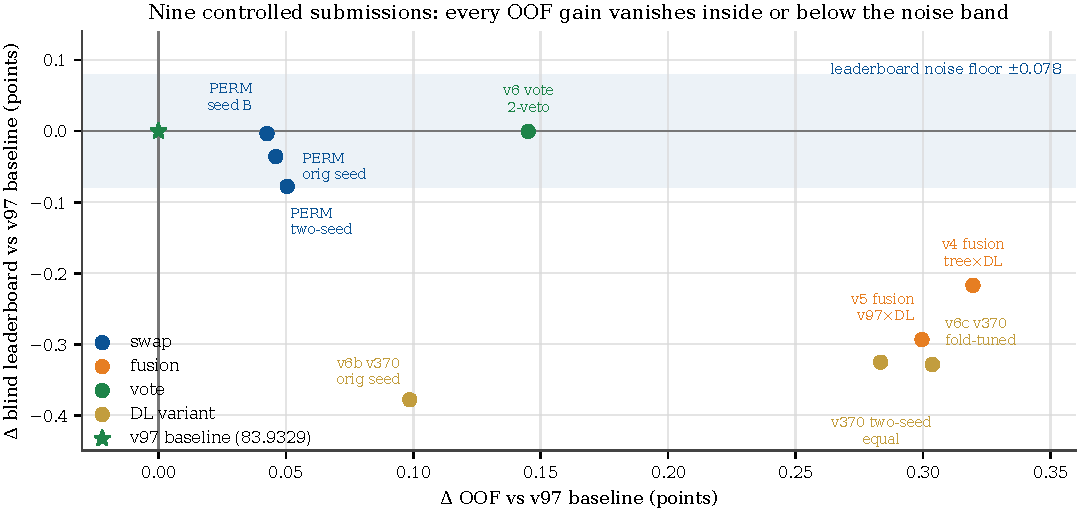
\includegraphics[width=\textwidth]{figures/fig13_submissions_chain.pdf}
\caption{Nine controlled submissions: every OOF gain vanishes inside or below the noise band. Each point is a submission's change over the v97 baseline in OOF (x) versus blind leaderboard (y); colours distinguish single-head swaps (blue), posterior fusions (orange), majority votes (green) and standalone DL variants (gold); the star marks the v97 baseline; the shaded band denotes the leaderboard's own noise floor $\pm$0.078 measured in \S\ref{sec:paradox}.}
\label{fig:submissions-chain}
\end{figure}

With fifty-thousand-wells-class training data and ten blind wells, the blind side acts like its own distribution, in which blind-set credit goes to the prediction morphology that the baseline already produces at those wells; any improvement that touches that morphology---including a drift-resilient gate that repairs the diagnosed failure mechanism and measures +1.36 SW under honest drift---simply is not what the five blind wells reward. No further in-province candidate amendment (posteriores, votes, seed ensembles, fold-tuned weights, decision-layer tweaks) remained untried; a next model-line must either be a new, drift-aware model built from the ground up or a preserved baseline.

\section{Type-well selection and DTW alignment on the 80-well benchmark}
\label{sec:typewell}

The 2021 SPWLA PDDA contest on Volve data was won by ``type-well'' adaptation: each test well is paired with the training wells that are statistically closest to it (KL divergence, DTW), and simple models are fitted on those wells only \cite{fu2024contest}. We tested this family on our benchmark with the four similarity criteria of Section~\ref{sec:alignment_methods}.

\paragraph{Selection criteria disagree} The eight nearest wells chosen by the four criteria overlap only weakly (mean top-8 overlap 0.13 between GR-DTW and median-curve distance, 0.16 between GR-DTW and KL, 0.29 between KL and median-curve distance, 0.33 between the two DTW variants), so ``the similar wells'' is not a well-defined set on this data.

\paragraph{No criterion beats pooling} Table~\ref{tab:typewell} and Fig.~\ref{fig:typewell} give leave-well-out accuracies (LightGBM, 16 evaluation wells) when training on the 12 or 30 nearest wells, on all 79 wells with similarity weights $\exp(-d/\mathrm{median}\,d)$, and on all 79 wells unweighted. KL divergence is the best criterion (POR 0.302 with 12 wells against 0.242 for median-curve distance), confirming the winning team's choice of statistic, but every restricted or weighted training set is at best equal to unweighted pooling (POR 0.315--0.326 vs 0.322; SW 0.126--0.137 vs 0.134).

\begin{table}[t]
\centering
\caption{Type-well selection on the 80-well benchmark: leave-well-out official accuracy on non-default samples (LightGBM on 13 curves + depth, 16 evaluation wells) by similarity criterion and training-set rule.}
\label{tab:typewell}
\small
\resizebox{\textwidth}{!}{%
\begin{tabular}{l l ccc c}
\toprule
Target & Criterion & 12 nearest & 30 nearest & All 79, similarity-weighted & All 79, unweighted \\
\midrule
POR & median-curve distance & 0.242 & 0.293 & 0.315 & 0.322 \\
POR & KL divergence & 0.302 & 0.307 & 0.323 & 0.322 \\
POR & GR DTW & 0.271 & 0.299 & 0.326 & 0.322 \\
POR & composite DTW & 0.287 & 0.306 & 0.317 & 0.322 \\
SW & median-curve distance & 0.132 & 0.137 & 0.134 & 0.134 \\
SW & KL divergence & 0.127 & 0.133 & 0.135 & 0.134 \\
SW & GR DTW & 0.128 & 0.134 & 0.130 & 0.134 \\
SW & composite DTW & 0.132 & 0.126 & 0.136 & 0.134 \\
\bottomrule
\end{tabular}}
\end{table}

\begin{figure}[t]
\centering
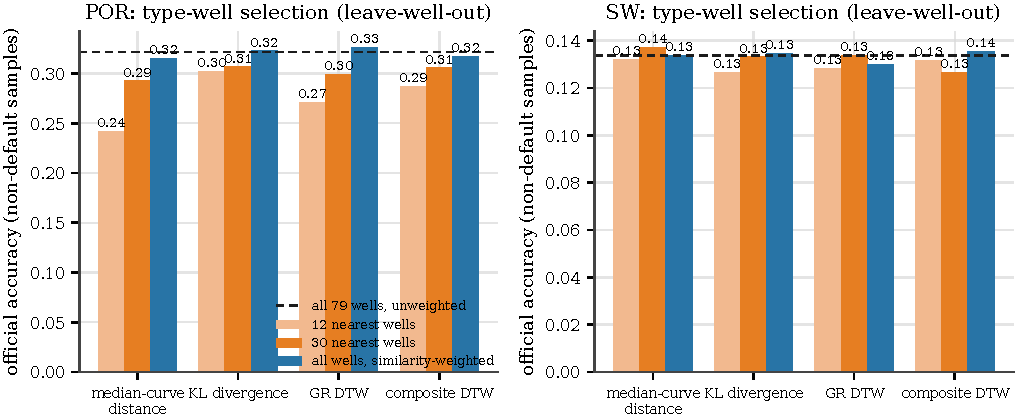
\includegraphics[width=\textwidth]{figures/fig8_typewell.pdf}
\caption{Type-well selection on the 80-well benchmark (leave-well-out, non-default samples). Four similarity criteria, training on the 12 or 30 nearest wells or on all wells with similarity weights, against training on all 79 wells (dashed line). No criterion or rule beats pooling.}
\label{fig:typewell}
\end{figure}

\paragraph{Alignment features carry structure, not values} Copying the interpreted labels of the eight DTW-aligned neighbour wells directly as a prediction identifies reservoir versus non-reservoir samples with 80--81\,\% accuracy but scores only 0.055 (POR) and 0.074 (SW) on non-default samples; the transferred information is where reservoirs are, which the models already know (gate accuracy 0.92--0.93). Accordingly, adding the 17 alignment features to the distribution models, the gates and the state model changes every score by at most 0.001 (POR joint-decoded 0.7845 $\to$ 0.7847, SW 0.7494 $\to$ 0.7493, PERM 0.8982 $\to$ 0.8979, state accuracy 0.9053 $\to$ 0.9060), and the fusion that includes them scores 81.642 against 81.632 without them.

%% =====================================================================
\section{Transfer to the SPWLA PDDA 2021 Volve benchmark}
\label{sec:transfer}

To test whether the conclusions depend on one basin and one metric, the pipeline was re-run without modification of its logic on the public SPWLA PDDA 2021 contest data \cite{pddasig2021,fu2024contest}, derived from the Equinor Volve field \cite{volve2018}: nine training wells (318,967 samples, 42,309 of them with the three interpreted targets porosity PHIF, water saturation SW and shale volume VSH, all in $[0,1]$), four blind wells with released truth (11,275 samples), and a root-mean-square-error (RMSE) metric over the three targets. The Volve curves were mapped onto the competition curve names with unit conversions (depth ft$\to$m, DTC $\mu$s/ft$\to\mu$s/m, calliper and bit size inch$\to$cm, neutron fraction$\to$\%); SP, deviation and azimuth do not exist there and enter as constant features. Water saturation has a mass point at SW = 1 (41\,\% of the labelled training samples, 52\,\% of the blind samples) that plays the role of the default value; PHIF and VSH have none.

\begin{table}[t]
\centering
\caption{Volve transfer experiment. Left: leave-well-out cross-validation over the nine training wells (labelled samples only). Right: the four blind wells with released truth. RMSE is the contest metric over the three targets; ``tol.'' is the tolerance accuracy of Section~\ref{sec:metric} applied to PHIF (8\,\%).}
\label{tab:volve}
\small
\resizebox{\textwidth}{!}{%
\begin{tabular}{l cc cc cc}
\toprule
 & \multicolumn{2}{c}{Leave-well-out CV} & \multicolumn{2}{c}{+ SW = 1 gate (CV)} & \multicolumn{2}{c}{Blind wells} \\
Model & RMSE & tol.\ PHIF & CatBoost gate & network gate & RMSE & tol.\ PHIF \\
\midrule
Tutorial Random Forest (five logs) & -- & -- & -- & -- & 0.1108 & -- \\
CatBoost RMSE regression, 294 features & 0.0661 & 0.424 & \textbf{0.0581} & 0.0596 & 0.1079 & 0.409 \\
\quad + CatBoost SW = 1 gate, threshold 0.5 & & & & & \textbf{0.1061} & \\
60-bin distributions, mean decoding & 0.0907 & 0.396 & 0.0624 & 0.0709 & 0.1185 & 0.487 \\
60-bin distributions, Bayes-action decoding & 0.0807 & \textbf{0.474} & 0.0687 & 0.0737 & 0.1148 & \textbf{0.516} \\
Sequence network alone (42k labelled samples) & 0.2326 & 0.061 & 0.1987 & 0.2312 & 0.1532 & 0.111 \\
\midrule
Contest leaderboard: 1st / 2nd / 3rd & & & & & 0.0525 / 0.0602 / 0.0634 & \\
\bottomrule
\end{tabular}}
\end{table}

Table~\ref{tab:volve} summarises the outcome. (i) \emph{Decoding follows the metric.} Under RMSE the mean-decoded distribution model beats the Bayes-action decoding (0.0907 vs 0.0807 is reversed in favour of the mean once the gate is added: 0.0624 vs 0.0687), whereas under the tolerance metric the Bayes action is best (0.474 vs 0.396 vs 0.424 for regression) -- the same model serves both metrics if the decoder is chosen accordingly. (ii) \emph{Pooling beats nearest-well training also on Volve.} In the Volve identifiability audit the same-well half split gives RMSE 0.141 for SW against 0.088 for cross-well training and 0.165 for the two nearest wells; for VSH 0.074 / 0.078 / 0.096; porosity is essentially density porosity everywhere (0.020 / 0.021 / 0.020). (iii) \emph{The network's segmentation advantage does not transfer with 42k labelled samples}: its SW = 1 gate accuracy is 0.68 against 0.90 for CatBoost, and it hurts every fusion. (iv) \emph{Blind wells expose a distribution shift the pooled model cannot absorb.} The best configuration scores 0.106, at the level of the tutorial baseline and twice the winning 0.0525, although three of the four wells score 0.051--0.125 (well 15/9-F-15: 0.051, at the winners' level). Well 15/9-F-11T2 is 97.6\,\% water (SW = 1) while no training well exceeds 92\,\%, its gate accuracy is 0.65, and it alone lifts the total RMSE to 0.144; the third-placed team set this whole well to SW = 1 by a well-level resistivity rule and the winner reached a similar effect through type-well adaptation \cite{fu2024contest}. With nine training wells, strong inter-well calibration drift and blind wells outside the training range, well-level adaptation is worth more than model capacity; with 80 wells from one basin the opposite holds (Section~\ref{sec:typewell}).

%% =====================================================================
\section{Discussion}

The five results sections line up as two lessons of different kinds. Within-family, needle-in-haystack gains of structure are real: the identifiability ceiling of \S\ref{sec:audit} (36--42\,\%) bounds what the logs carry, and the tolerance-aligned decoding, joint state variable and whole-well CNN of \S\ref{sec:methods} lift the official progression from 80.88 to 81.63, an improvement that transfers cleanly to the same blind wells (82.27 $\to$ 83.26) with exactly additive ablation deltas (+0.720 gates +0.266 values). Type-well selection and DTW alignment, although state of the practice on single-basin petrology, do not help at this scale; their transfer conditions are quantified on the public Volve benchmark.

Across-family, the same reasoning fails in a second way. The newer 8-stage chain improves honest OOF total (+0.283) yet scores below the older 18-stage chain at the blind wells by several times the measured noise floor ($-$0.325 with a $\pm$0.04--0.08 band); degradation stacks in the SW head whose default decisions flip most under the raw curve shifts recorded in \S\ref{sec:drift}. The blind wells are not outliers in input space (mean per-curve KS 0.114--0.240, matching the pool's natural variation), yet blind-set credit accrues to the older chain's exact morphology so exclusively that nine further OOF-positive submissions measure themselves below the baseline with only the minimal-morphology variant (2.2\,\% of rows) reaching a tie within the noise band. The B' repair motivated by the diagnosis does work---label-preserving per-well curve perturbations collapse the SW gate's drift sensitivity by about 95\,\% and a gate-on-value transplant measures +1.36 on SW under drift---while remaining unpriced by a five-well leaderboard designed to score only well-level similarity.

The lesson is joint: identifiability limits what logs can carry, tolerance-aligned decoding is needed to read it, division of labour beats one-model thinking, and well-level drift is where distribution-aware care outperforms careful models. Type-well selection, DTW alignment, posterior fusions and majority votes each have their own formal conditions of paying; with the benchmark blind wells already being ordinary out-of-fold wells in input space, none of those conditions applies at the leaderboard level, and no in-province amendment can lift the score while preserving the morphology that the score rewards.

\section{Conclusions}

On a 90-well wireline-log benchmark scored by a relative-tolerance metric, the amount of interpreted-label variation recoverable from the input curves alone is bounded by a measured identifiability ceiling of 36--42\,\%, owing to zonation and core-calibration information absent from the curves. Within that ceiling, structural decisions beat tuning: tolerance-aligned Bayes-action decoding of binned distributions, a jointly modelled reservoir-state variable, and a whole-well CNN whose segmentation gains are additive to those of trees, lifting cross-validation from 80.88 to 81.63 and the blind wells from 82.27 to 83.26, with additive ablation deltas (+0.720 gates, +0.266 values). Type-well selection, DTW alignment and Volve-transfer experiments complete the first model family's picture: these techniques have their own conditions, and this benchmark is not among them.

The deeper lesson comes from testing the same benchmark with a second model family: once blind-set resolution matters, the leaderboard defends morphology rather than ranking in-distribution improvements. Every measured OOF gain of the newer chain---searches of architecture, seeds, weights, votes, fusions and a drift-repair of the exact component diagnosed as the drift failure carrier---does not pay at the five blind wells, under a measured blind noise floor of $\pm$0.04--0.08 against in-distribution gains of up to +0.58. Since the blind wells are ordinary out-of-fold wells in input space (§\ref{sec:drift}), the bottleneck is not input-domain outliers: it is that blind-set credit scores the rows where prediction morphology matches the current leader, and every in-province candidate touches those rows.

The project also contributes a directly usable method: label-preserving per-well curve perturbations calibrated to measured well-level drift, which collapse the drift sensitivity of the vulnerable model head by about 95\,\% at a cost of roughly 0.1 official clean-OOF points and are the first step we now take whenever blind-set drift is measured before deciding to train, transplant, or simply preserve. Code, machine-readable evidence sets, all per-version prediction artifacts and the complete submission codepackages of v4--v7 are released at the repository; every number in this paper is reconstructible end-to-end from the preserved artifacts.

\section*{Declaration of generative AI and AI-assisted technologies in the manuscript preparation process}
During the preparation of this work the authors used an AI coding assistant (Claude, Anthropic) to draft analysis code, run experiments under the authors' specification, and produce a first draft of the text. After using this tool the authors reviewed and edited the content as needed and take full responsibility for the content of the published article.

\section*{Declaration of competing interest}
The authors declare that they have no known competing financial interests or personal relationships that could have appeared to influence the work reported in this paper.

\section*{Data availability}
The benchmark data are the property of the competition organiser; access conditions are described at [URL]. The Volve-based SPWLA PDDA 2021 data are public \cite{pddasig2021}. Code for all experiments (feature construction, CatBoost and network training, decision layer, nested fusion, diagnostics, transfer experiment), the out-of-fold experiment registry, the per-well scores and the well-similarity matrices are provided as supplementary material and will be deposited at [Mendeley Data / repository DOI].

In addition, the newer experiment families are archived under \texttt{results/dl\_fusion/} (DL-family weight grids, nested CV, per-row dumps and drift descriptor sets), \texttt{results/drift\_sw/} (drift-augmentation: two-arm ablations, calibration mappings, sensitivity and transplant details) and \texttt{results/dl\_fusion/drift/} (test-versus-train and leave-one-out inter-well drift descriptors). Blind leaderboard entries are tagged in each \texttt{submissions/v*/manifest.json}. Figures~9--13 and the restyled versions of Figures~1--8 were regenerated with \texttt{solution\_v7/fig\_rebuild\_1\_8.py} and \texttt{solution\_v7/fig\_new\_9\_13.py} from the archived JSON evidence; CSV snapshots of each figure are kept in \texttt{docs/figures/}. All inference runs on H20 hardware are deterministic and sealed by SHA256 manifests (\texttt{RUNTIME\_PINNING.json}).

\section*{Funding}
This research did not receive any specific grant from funding agencies in the public, commercial, or not-for-profit sectors.

\bibliographystyle{elsarticle-num}
\bibliography{refs}

\end{document}
